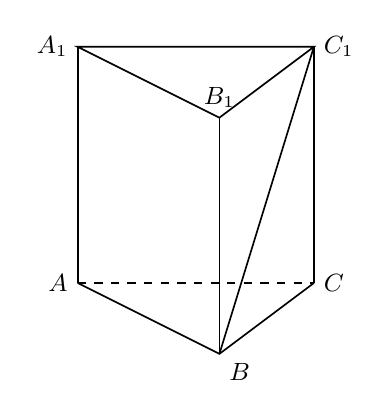
\begin{tikzpicture}[line width=0.6pt, font=\small]
  \coordinate (A) at (0,0);
  \coordinate (C) at (3,0);
  \coordinate (B) at (1.8,-0.9);
  \coordinate (A1) at (0,3);
  \coordinate (C1) at (3,3);
  \coordinate (B1) at (1.8,2.1);
  % Vertical edges solid
  \draw (A) -- (A1);
  \draw (B) -- (B1);
  \draw (C) -- (C1);
  % Top triangle solid
  \draw (A1) -- (B1) -- (C1) -- cycle;
  % Bottom: front solid, back dashed
  \draw (A) -- (B) -- (C);
  \draw[dashed] (A) -- (C);
  % Diagonal BC1 (the line in question) solid
  \draw (B) -- (C1);
  % Labels
  \node[left] at (A1) {$A_{1}$};
  \node[left] at (A) {$A$};
  \node[right] at (C1) {$C_{1}$};
  \node[right] at (C) {$C$};
  \node[below right] at (B) {$B$};
  \node[above] at (B1) {$B_{1}$};
\end{tikzpicture}
